% !TeX spellcheck = cs_CZ
% Marsak, Havrankova - Sbirka resenych prikladu z fyziky - Termika a molekulova fyzika.pdf
\begin{example}\label{fyz:fey_exam011}
  Lampa o hmotnosti \SI{5}{\kg} visí uprostřed dlouhého původně vodorovného drátu a způsobí jeho 
  prohnutí o \ang{1} od vodorovného směru (viz obr. \ref{fyz:fig379}). Určete velikost síly \(F_n\)
  napínající drát. 
      
  {\centering
   \captionsetup{type=figure}
   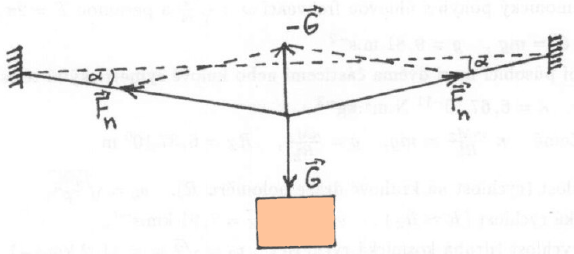
\includegraphics[width=0.7\linewidth]{fyz_fig379.png}
   \captionof{figure}{K příkladu \ref{fyz:fey_exam011} \cite[s.~6]{Havrankova1995}
   \label{fyz:fig379}}
  \par}
  
  Tíhová síla, kterou lampa prohýbá drát musí být vyrovnána vertikální silou vzniklou jako 
  výslednice napěťových sil působících v drátu. Tedy
  \begin{equation*}
     G = 2F_n\sin\alpha = mg, \quad m = \SI{5}{\kg}, \quad
     \sin\alpha = \sin\ang{1} \approx \alpha = \num{0.017}
  \end{equation*}
  \begin{equation*}
    F_n = \frac{mg}{2\sin\alpha} = \frac{\num{5}\cdot\num{9.81}}{2\cdot\num{0.017}}
        = \SI{1443}{\newton}
  \end{equation*}
  \begingroup\makeatletter\def\f@size{7}\check@mathfonts
  \def\maketag@@@#1{\hbox{\m@th\large\normalfont#1}}%
    \begin{align*}
      \shortintertext{\footnotesize Použitý vzorec můžeme snadno odvodit z kosinové věty:}
      G &= \sqrt{F_1^2 + F_2^2 - 2F_1F_2\cdot\cos2\alpha} \\
      \shortintertext{\footnotesize s přihlédnutím, že obě síly jsou si rovny a s využitím  
        goniometrického vzorce pro dvojnásobný úhel \(\cos2\alpha = \cos^2\alpha - \sin^2\alpha\) 
        můžeme provést následující úpravy} 
      G &= \sqrt{2F_n^2\cdot(1-\cos2\alpha)}=\sqrt{2}F_n\sqrt{1-\cos^2\alpha+\sin^2\alpha}  \\
        &=\sqrt{2}F_n\sqrt{2\sin^2\alpha} = 2F_n\sin\alpha
    \end{align*}
  \endgroup
  Drát bude napínán stejnou silou, jako kdyby na něj působilo tahem těleso tíhy \SI{1443}{\newton}, 
  tedy o hmotnosti \SI{147}{\kg}
\end{example}